\section{Структура операционной системы}\label{base:os:structure}
\emph{Операционная система} --- сложный комплекс разнообразных программ, с одной стороны являющихся интерфейсом между устройствами вычислительной системы и прикладными программами, а с другой --- предназначенных для управления устройствами, управления вычислительными процессами, эффективного распределения вычислительных ресурсов между вычислительными процессами и организации надёжных вычислений.

\subsection{Ядро}\label{base:os:structure:kernel}
Ядро --- центральная часть операционной системы (ОС), обеспечивающая приложениям координированный доступ к ресурсам компьютера, таким как процессорное время, память, внешнее аппаратное обеспечение, внешнее устройство ввода и вывода информации. Также обычно ядро предоставляет сервисы файловой системы и сетевых протоколов.

Как основополагающий элемент ОС, ядро представляет собой наиболее низкий уровень абстракции для доступа приложений к ресурсам системы, необходимым для их работы. Как правило, ядро предоставляет такой доступ исполняемым процессам соответствующих приложений за счёт использования механизмов межпроцессного взаимодействия и обращения приложений к системным вызовам ОС.

Описанная задача может различаться в зависимости от типа архитектуры ядра и способа её реализации.

\subsubsection{Типы архитектур ядер операционных систем}\label{base:os:structure:kernel:types}
\paragraph{Монолитное.} Классическая и, на сегодняшний день, наиболее распространённая архитектура ядер операционных систем --- это \emph{монолитные} ядра. Они предоставляют богатый набор абстракций оборудования. Все части монолитного ядра работают в одном адресном пространстве.

Монолитные ядра имеют долгую историю развития и усовершенствования и, на данный момент, являются наиболее архитектурно зрелыми и пригодными к эксплуатации. Вместе с тем, монолитность ядер усложняет их отладку, понимание кода ядра, добавление новых функций и возможностей, удаление <<мёртвого>>, ненужного, унаследованного от предыдущих версий кода. <<Разбухание>> кода монолитных ядер также повышает требования к объёму оперативной памяти, требуемому для функционирования ядра ОС. Это делает монолитные ядерные архитектуры малопригодными к эксплуатации в системах, сильно ограниченных по объёму ОЗУ, например, встраиваемых системах, производственных микроконтроллерах и~т.\,д..

\paragraph{Модульное.} Ограниченность и громоздкость монолитных ядер привели к появлению т.\,н.~\emph{модульных} ядер.

В отличие от <<классических>> монолитных ядер, считающихся ныне устаревшими, модульные ядра, как правило, не требуют полной перекомпиляции ядра при изменении состава аппаратного обеспечения компьютера. Вместо этого модульные ядра предоставляют тот или иной механизм подгрузки модулей ядра, поддерживающих то или иное аппаратное обеспечение (например, драйверов).
При этом подгрузка модулей может быть как динамической (выполняемой <<на лету>>, без перезагрузки ОС, в работающей системе), так и статической (выполняемой при перезагрузке ОС после переконфигурирования системы на загрузку тех или иных модулей).

Все модули ядра работают в адресном пространстве ядра и могут пользоваться всеми функциями, предоставляемыми ядром. Поэтому модульные ядра продолжают оставаться монолитными. Модульность ядра осуществляется на уровне бинарного образа, а не на архитектурном уровне ядра, так как динамически подгружаемые модули загружаются в адресное пространство ядра и в дальнейшем работают как интегральная часть ядра.
Модульные монолитные ядра не следует путать с архитектурным уровнем модульности, присущий микроядрам и гибридным ядрам. Практически, динамичная загрузка модулей, это просто более гибкий способ изменения образа ядра во время выполнения — в отличие от перезагрузки с другим ядром. Модули позволяют легко расширить возможности ядра по мере необходимости.

Модульные ядра удобнее для разработки, чем традиционные монолитные ядра, не поддерживающие динамическую загрузку модулей, так как от разработчика не требуется многократная полная перекомпиляция ядра при работе над какой-либо его подсистемой или драйвером. Выявление, локализация, отладка и устранение ошибок при тестировании также облегчаются.

Модульные ядра предоставляют особый программный интерфейс (API) для связывания модулей с ядром, для обеспечения динамической подгрузки и выгрузки модулей. В свою очередь, не любая программа может быть сделана модулем ядра: на модули ядра накладываются определённые ограничения в части используемых функций (например, они не могут пользоваться функциями стандартной библиотеки С/С++ и должны использовать специальные аналоги, являющиеся функциями API ядра).
Кроме того, модули ядра обязаны экспортировать определённые функции, нужные ядру для правильного подключения и распознавания модуля, для его корректной инициализации при загрузке и корректного завершения при выгрузке, для регистрации модуля в таблице модулей ядра и для обращения из ядра к сервисам, предоставляемым модулем.

Не все части ядра могут быть сделаны модулями. Некоторые части ядра всегда обязаны присутствовать в оперативной памяти и должны быть жёстко <<вшиты>> в ядро. Также не все модули допускают динамическую подгрузку (без перезагрузки ОС).
Общей тенденцией развития современных модульных ядер является всё большая модуляризация кода, улучшение механизмов динамической подгрузки и выгрузки, уменьшение или устранение необходимости в ручной подгрузке модулей или в переконфигурации ядра при изменениях аппаратуры путём введения тех или иных механизмов автоматического определения оборудования и автоматической подгрузки нужных модулей, универсализация кода ядра и введение в ядро абстрактных механизмов, предназначенных для совместного использования многими модулями. Примером может служить VFS --- <<виртуальная файловая система>>, совместно используемая многими модулями файловых систем в ядре Linux.

\paragraph{Микроядро.} \emph{Микроядро} --- это минимальная реализация функций ядра операционной системы.

Классические микроядра предоставляют лишь очень небольшой набор низкоуровневых примитивов, или системных вызовов, реализующих базовые сервисы операционной системы.

К ним относятся:
\begin{itemize}
 \item управление адресным пространством оперативной памяти.
 \item управление адресным пространством виртуальной памяти.
 \item управление процессами и потоками (нитями).
 \item средства межпроцессной коммуникации.
\end{itemize}

Все остальные сервисы ОС, в классических монолитных ядрах предоставляемые непосредственно ядром, в микроядерных архитектурах реализуются в адресном пространстве пользователя (Ring3) и называются сервисами. Примерами таких сервисов, выносимых в пространство пользователя в микроядерных архитектурах, являются сетевые сервисы, файловая система, драйверы.

Основное достоинство микроядерной архитектуры --- высокая степень модульности ядра операционной системы. Это существенно упрощает добавление в него новых компонентов. В микроядерной операционной системе можно, не прерывая её работы, загружать и выгружать новые драйверы, файловые системы и~т.\,д.. Существенно упрощается процесс отладки компонентов ядра, так как новая версия драйвера может загружаться без перезапуска всей операционной системы.
Компоненты ядра операционной системы ничем принципиально не отличаются от пользовательских программ, поэтому для их отладки можно применять обычные средства. Микроядерная архитектура повышает надежность системы, поскольку ошибка на уровне непривилегированной программы менее опасна, чем отказ на уровне режима ядра. И чтобы добавить в ОС с микроядром драйвер того или иного устройства, не надо перекомпилировать всё ядро, а надо лишь отдельно откомпилировать этот драйвер и запустить его в пользовательском пространстве.

В то же время микроядерная архитектура операционной системы вносит дополнительные накладные расходы, связанные с обменом сообщениями, что отрицательно влияет на производительность. Для того чтобы микроядерная операционная система по скорости не уступала операционным системам на базе монолитного ядра, требуется очень аккуратно проектировать разбиение системы на компоненты, стараясь минимизировать взаимодействие между ними. Таким образом, основная сложность при создании микроядерных операционных систем --- необходимость очень аккуратного проектирования.

Микроядра типа ядра ОС Minix и GNU Hurd развиваются медленно, гораздо медленнее, чем Linux и ядро систем семейства BSD. По словам создателя Minix3, Таненбаума, он пытается <<построить сверхнадёжную систему. Она может использоваться в том числе на серверах, которым необходимы годы безотказной работы>>.

Классическим примером микроядерной системы является Symbian OS. Это пример распространенной и отработанной микроядерной (a начиная c версии Symbian OS v8.1, и наноядерной) операционной системы. Создателям Symbian OS удалось совместить эффективность и концептуальную стройность, несмотря на то что современные версии этой системы предоставляют обширные возможности, в том числе средства для работы c потоковыми данными, стеками протоколов, критичными к латентности ядра, графикой и видео высокого разрешения).
Разработчики Symbian вынесли практически все прикладные (т.e. выходящие за пределы компетенции ядра) задачи в модули-серверы, функционирующие в пользовательском адресном пространстве.

В ОС Windows NT версий 3.х микроядерная архитектура с сервисным процессом использовалась для подсистемы графики и пользовательского интерфейса. В частности, драйвер графической аппаратуры загружался в контекст сервисного процесса, а не ядра.
Начиная с версии 4, от этого отказались, сервисный процесс сохранился только для управления консольными окнами командной строки, а собственно графическая подсистема вместе с драйвером аппаратуры (в том числе трехмерной графики) переместилась в специально обособленный регион ядра ОС.

ОС Windows CE (и созданные на её основе сборки, такие, как Windows Mobile), будучи практически полностью совместимой (как подмножество) с Windows NT по вызовам и методам программирования приложений, тем не менее полностью отличается от Windows NT по внутренней архитектуре и является микроядерной ОС с выносом всех драйверов устройств, сетевых стеков и графической подсистемы в сервисные процессы.

Недостаток --- плата за принудительное «переключение» процессов в ядре (переключение контекста); этот факт собственно и объясняет трудности в проектировании и написании ядер подобной конструкции. Эти недостатки способны обойти ОС, использующие архитектуру экзоядра, являющуюся дальнейшим развитием микроядерной архитектуры.

\paragraph{Экзоядро.} В традиционных операционных системах ядро предоставляет не только минимальный набор сервисов, обеспечивающих выполнение программ, но и большое количество высокоуровневых абстракций для использования разнородных ресурсов компьютера: оперативной памяти, жестких дисков, сетевых подключений.
В отличие от них, ОС на основе \emph{экзоядра} предоставляет лишь набор сервисов для взаимодействия между приложениями, а также необходимый минимум функций, связанных с защитой: выделение и высвобождение ресурсов, контроль прав доступа, и~т.\,д. Экзоядро не занимается предоставлением абстракций для физических ресурсов --- эти функции выносятся в библиотеку пользовательского уровня (так называемую libOS).

Основная идея операционной системы на основе экзоядра состоит в том, что ядро должно выполнять лишь функции координатора для небольших процессов, связанных только одним ограничением --- экзоядро должно иметь возможность гарантировать безопасное выделение и освобождение ресурсов оборудования.
В отличие от ОС на основе микроядра, ОС, базирующиеся на экзоядре, обеспечивают гораздо большую эффективность за счет отсутствия необходимости в переключении между процессами при каждом обращении к оборудованию.

Архитектуры на основе экзоядер являются дальнейшим развитием и усовершенствованием микроядерных архитектур и одновременно ужесточают требования к минималистичности и простоте кода ядра. libOS может обеспечивать произвольный набор абстракций, совместимый с той или иной уже существующей операционной системой, например GNU/Linux или Windows.

\paragraph{Наноядро.} \emph{Наноядро} --- архитектура ядра операционной системы компьютеров, в рамках которой крайне упрощённое и минималистичное ядро выполняет лишь одну задачу --- обработку аппаратных прерываний, генерируемых устройствами компьютера.
После обработки прерываний от аппаратуры наноядро, в свою очередь, посылает информацию о результатах обработки (например, полученные с клавиатуры символы) вышележащему программному обеспечению при помощи того же механизма прерываний. Также часто реализуют минимальную поддержку потоков:~создание и переключение.

В некотором смысле концепция наноядра близка к концепции HAL --- Hardware Abstraction Layer, предоставляя вышележащему ПО удобные механизмы абстракции от конкретных устройств и способов обработки их прерываний.

Наиболее часто в современных компьютерах наноядра используются для виртуализации аппаратного обеспечения реальных компьютеров или для реализации механизма гипервизора, с целью позволить нескольким или многим различным операционным системам работать одновременно и параллельно на одном и том же компьютере.
Например, VMware ESX Server реализует собственное наноядро, не зависимое от ОС и устанавливаемое на <<голое железо>>. Поверх этого наноядра работают пользовательские и административные утилиты VMware и сами операционные системы, виртуализируемые в ESX Server.

Наноядра также могут использоваться для обеспечения переносимости (портабельности) операционных систем на разное аппаратное обеспечение или для обеспечения возможности запуска <<старой>> операционной системы на новом, несовместимом аппаратном обеспечении без её полного переписывания и портирования.
Например, фирма Apple Computer использовала наноядро в версии Mac OS Classic для PowerPC для того, чтобы транслировать аппаратные прерывания, генерировавшиеся их компьютерами на базе процессоров PowerPC в форму, которая могла <<пониматься>> и распознаваться Mac OS для процессоров Motorola 680x0. Таким образом, наноядро эмулировало для Mac OS <<старое>> 680x0 железо.
Альтернативой было бы полное переписывание и портирование кода Mac OS на PowerPC при переходе с 680x0 на них. Позднее, в эпоху Mac OS 8.6, наноядро виртуализировало предоставляемые PowerPC мультипроцессорные возможности и обеспечивало поддержку SMP в Mac OS.
Другие удачные примеры использования наноядерных архитектур включают наноядро Adeos, работающее как модуль ядра для Linux и позволяющее выполнять одновременно с Linux какую-либо операционную систему реального времени.

Наноядро может быть настолько маленьким и примитивным, что даже важнейшие устройства, находящиеся непосредственно на материнской плате или на плате контроллера встраиваемого устройства, такие, как таймер или программируемый контроллер прерываний, обслуживаются специальными драйверами устройств, а не непосредственно ядром. Такого рода сверхминималистичные наноядра называют иногда пикоядрами.

Термин <<наноядро>> иногда неформально используется для описания очень маленьких, упрощённых и лёгких микроядер, таких, как L4.

\paragraph{Гибридное ядро.} \emph{Гибридное ядро} --- модифицированные микроядра (минимальная реализация основных функций ядра операционной системы компьютера), позволяющие для ускорения работы запускать <<несущественные>> части в пространстве ядра.

Все рассмотренные подходы к построению операционных систем имеют свои достоинства и недостатки. В большинстве случаев современные операционные системы используют различные комбинации этих подходов. 
Так, например сейчас, Linux представляет собой монолитную систему с отдельными элементами модульного ядра. При компиляции ядра можно разрешить динамическую загрузку и выгрузку очень многих компонентов ядра --- так называемых модулей.
В момент загрузки модуля его код загружается на уровне системы и связывается с остальной частью ядра. Внутри модуля могут использоваться любые экспортируемые ядром функции.

Существуют варианты ОС GNU (Debian GNU/Hurd), в которых вместо монолитного ядра применяется ядро Mach (такое же, как в Hurd), а поверх него в пользовательском пространстве работают те же самые процессы, которые при использовании Linux были бы частью ядра.
Другим примером смешанного подхода может служить возможность запуска операционной системы с монолитным ядром под управлением микроядра. Так устроены 4.4BSD и MkLinux, основанные на микроядре Mach.
Микроядро обеспечивает управление виртуальной памятью и работу низкоуровневых драйверов. Все остальные функции, в том числе взаимодействие с прикладными программами, осуществляется монолитным ядром. Данный подход сформировался в результате попыток использовать преимущества микроядерной архитектуры, сохраняя по возможности хорошо отлаженный код монолитного ядра.

Наиболее тесно элементы микроядерной архитектуры и элементы монолитного ядра переплетены в ядре Windows NT. Хотя Windows NT часто называют микроядерной операционной системой, это не совсем так. 
Микроядро NT слишком велико (более 1 Мбайт, кроме того, в ядре системы находится, например, ещё и модуль графического интерфейса), чтобы носить приставку <<микро>>. Компоненты ядра Windows NT располагаются в вытесняемой памяти и взаимодействуют друг с другом путем передачи сообщений, как и положено в микроядерных операционных системах.
В то же время все компоненты ядра работают в одном адресном пространстве и активно используют общие структуры данных, что свойственно операционным системам с монолитным ядром. Причина проста: чисто микроядерный дизайн коммерчески менее выгоден, поскольку менее эффективен (за счет накладных расходов на передачу сообщений там, где можно было обойтись вызовами функций).Таким образом, Windows NT можно с полным правом назвать гибридной операционной системой.

Смешанное ядро, в принципе, должно объединять преимущества монолитного ядра и микроядра: казалось бы, микроядро и монолитное ядро --- крайности, а смешанное --- золотая середина. В них возможно добавлять драйвера устройств двумя способами: и внутрь ядра, и в пользовательское пространство. Но на практике концепция смешанного ядра часто подчёркивает не только достоинства, но и недостатки обоих типов ядер.

\paragraph{Сравнение ядер различных типов.}
Приведём таблицу сравнения различных архитектур:
\newcolumntype{G}{>{\columncolor[rgb]{0, 1, 0}}c}
\newcolumntype{g}{>{\columncolor[rgb]{0.8, 1, 0.8}}p{4cm}}
\newcolumntype{B}{>{\columncolor[rgb]{1, 0, 0}}c}
\newcolumntype{b}{>{\columncolor[rgb]{1, 0.8, 0.8}}p{4cm}}
\def\tabrowsep{\noalign{\vskip 2pt}}
\begin{longtable}{lgb}
 Тип                         & \multicolumn{1}{G}{Достоинства} & \multicolumn{1}{B}{Недостатки} \\ \tabrowsep
 Монолитное & Скорость работы, упрощённая разработка модулей & Поскольку всё ядро работает в одном адресном пространстве, сбой в одном из компонентов может нарушить работоспособность всей системы, громоздкость \\ \tabrowsep
 Модульное & Те же, что у монолитного + большая гибкость & Те же, что у монолитного \\ \tabrowsep
 Микроядро & Устойчивость к сбоям оборудования, ошибкам в компонентах системы, упрощённое добавление новых компонентов и их отладки. & Передача данных между процессами требует накладных расходов. \\ \tabrowsep
 Экзоядро & Скорость, компактность, лёгкость разработки & --- \\ \tabrowsep
 Наноядро & Компактность, простая разработка & Ядро не предоставляет никаких механизмов для работы с железом, только простейшую обработку \\ \tabrowsep
 Гибридное ядро & Меньший размер, нежели у монолитного, большая скорость по сравнению с микроядром & Присущая монолитным ядрам громоздкость кода
\end{longtable}

\subsubsection{Некоторые примеры}\label{base:os:structure:kernel:examples}
\begin{itemize}
 \item Linux
 \item kFreeBSD
 \item Darwin
 \item Windows
 \item FreeDOS
 \item Mach
 \item Hurd
 \item QNX
\end{itemize}

\subsection{Средства загрузки и инициализации системы}\label{base:os:structure:bootandinit}
 Теперь давайте поговорим о том, что происходит во время загрузки. После инициализации оборудования BIOS передаёт управдение т.\,н. \emph{загрузочным устройствам} в порядке, указанном в настройках. Это могут быть оптические диски и прочие съёмные накопители, сетевые интерфейсы и, конечно же, внутренние жёсткие диски или аналогичные им устройства, такие как твердотельные накопители (SSD).
 При загрузке на устройстве ищется \emph{загрузочная область}, в которой располагается т.\,н.~ \emph{загрузчик}. Он нужен для того, чтобы загрузить ядро операционной системы и передать ему управление. После загрузки ядро инициирует аппаратное обеспечение, загружает \emph{средства инициализации системы} и передаёт им дальнейшее управление.
 
\subsubsection{Загрузчик}\label{base:os:structure:bootandinit:bootloader}
Применяется для загрузки ядра и передачи ему управления. В его задачи входит:
\begin{itemize}
 \item обеспечивание необходимых средств для диалога с пользователем (например, выбор операционной системы для загрузки);
 \item приведение аппаратуры компьютера в состояние, необходимое для старта ядра операционной системы;
 \item загрузка ядра операционной системы в ОЗУ;
 \item формирование параметров, передаваемых ядру операционной системы;
 \item передача управления ядру операционной системы.
\end{itemize}
 На компьютерах архитектуры IBM PC запуск загрузчика осуществляется программным обеспечением BIOS, записанной в ПЗУ компьютера, после успешного окончания процедуры POST. BIOS производит чтение 512 байт первого сектора жёсткого диска (MBR --- master boot record, основная загрузочная область) в ОЗУ, затем прочитанному коду передаётся управление.
 Этот код читает и анализирует таблицу разделов жёсткого диска, а затем, в зависимости от вида загрузчика, либо передаёт управление загрузочному коду активного раздела жёсткого диска, либо самостоятельно загружает ядро с диска в оперативную память и передаёт ему управление.
  
 Сам загрузчик может располагаться как в MBR, так и на разделах винтчестера. В последнем случае он не может быть загружен BIOS, поэтому ему передаётся управление от другого загрузчика. Цепочка, теоретически, может быть бесконечной, однако, т.\,к. в этом нет смысла, на практике используется один, реже два загрузчика. Важно, что только один загрузчик должен располагаться в MBR, т.\,к. попытка записать второй приведёт к тому, что первый будет перезаписан;
 также важно, что в MBR должен находиться загрузочный код (в случае, если загрузка происходит с жёсткого диска), иначе нечему будет передавать управление.
 
 \paragraph{LILO}
 Первым рассмотрим один из старейших загрузчиков --- \emph{LILO} (linux loader). 
 
 \paragraph{GRUB1}
 
 \paragraph{GRUB2}
 
 \paragraph{NTLDR}
  
\subsubsection{Средства инициализации системы}\label{base:os:structure:bootandinit:init}
После того, как загрузчик передал управление ядру и оно выполнило все необходимые действия, управление передаётся набору программ, отвечающих за запуск сервисов, различных систем, тесно работающих с ядром, предварительную подготовку оборудования (например, в случае использования зашифрованных разделов) и прочее.
Основным инструментом инициализации является программа \texttt{/sbin/init}, обеспечивающая упраление загрузкой, запуск других сервисов и являющаяся прямым или косвенным родительским процессом для всех запущенных приложений. Рассмотрим процесс инициализации поподробней:
  
Все современные системы инициализации имеют кое-что общее --- во всех есть программа \texttt{init}, все имеют список сервисов (в терминологии POSIX --- \emph{демонов}, англ. \emph{DAEMON}: disk and execution monitor), которые следует загрузить. Однако этот список организован по-разному. Существуют два основных типа систем инициализации --- \emph{BSD} и \emph{System V}.
  
\textbf{System V} (сокращённо \textbf{SysV}) является наиболее распространённым дизайном системы инициализации среди дистрибутивов GNU/Linux. В нём существует такое понятие, как \emph{уровни загрузки} (англ.\,\emph{run\-le\-vels}). Они позволяют загружать систему только с той функциональностью, которая нужна пользователю, например, без поддержки сети или в однопользовательском режиме для восстановления.
В SysV, если ядру не были переданы иные параметры, \texttt{init} изучает файл \texttt{/etc/inittab} на предмет наличия записи <<\texttt{:initdefault:}>>, которая указывает, какой уровень загрузки объявлен уровнем по-умол\-ча\-нию, и переходит на него, предварительно выполнив необходимые операции. Если уровень по-умолчанию не объявлен, пользователь должен выбрать его вручную в системной консоли.
Уровни загрузки, по сути, являются режимом, в который входит операционная система. Всего их, согласно спецификации стандарта LSB, 7:
 \begin{enumerate}
  \setcounter{enumi}{-1}
  \item \textbf{Halt}: выключение;
  \item \textbf{Single-user mode}: однопользовательский режим;
  \item \textbf{Multi-user mode}: многопользовательский режим;
  \item \textbf{Multi-user with networking}: многопользовательский режим с поддержкой сети;
  \item \textbf{User defined}: определяемый пользователем;
  \item \textbf{GUI}: многопользовательский режим с поддержкой сети и графическим интерфейсом
  \item \textbf{Reboot}: перезагрузка
 \end{enumerate}
Некоторые дистрибутивы могут использовать другие режимы, например, Debian использует дополнительный режим S для предварительной загрузки некоторых подсистем, хотя общая картина, обычно, не меняется. Узнать текущий уровень можно выполнив одну из следующих команд:\\
\texttt{\# runlevel}\\
\texttt{\$ who -r}\\
Изменить текущий уровень может суперпользователь, выполнив команду <<\texttt{init} \emph{уровень}>> или <<\texttt{telinit} \emph{уровень}>>.
 
Управление списком демонов на каждом уровне осуществляется путём помещения символической ссылки на скрипт, осуществляющий запуск демона, в соответствующую директорию. Скрипты лежат в директории \texttt{/etc/init.d/}, а уровни обычно представлены директориями с номером уровня загрузки \texttt{/etc/rc\{0-6\}.d/}
 
\textbf{BSD}-стиль используется в некоторых дистрибутивах GNU/Linux, а также в операционных системах семейства BSD. В отличие от SysV, здесь используется всего один файл, \texttt{/etc/rc.conf}, в котором указываются необходимые демоны. BSD-стиль обычно не предоставляет поддержки загрузочных уровней, но в дистрибутивах GNU/Linux разработчики совмещают оба подхода из соображений совместимости.
Скрипты находятся по адресу \texttt{/etc/rc.d/}; в отличие от SysV, где порядок выполнения скриптов определяется алфавитным порядком списка файлов в соответствующей директории, в BSD порядок определяется специальными метками, помещаемыми в каждый скрипт, либо порядком, в котором они указаны в файле \texttt{rc.conf}.
 
\subsection{Системные утилиты}\label{base:os:structure:sysutils}
Далее следуют утилиты поддержки функций ядра, обеспечивающие работу с устройствами, файловыми системами, сетевыми протоколами, средства управления модулями и многое другое. В POSIX-совместимых системах они находятся в директориях \texttt{/sbin/} (для минимальной системы) и \texttt{/usr/sbin/}. Далее мы будем рассматривать только программы из каталога \texttt{/sbin/}.

\subsubsection{Модули}\label{base:os:structure:sysutils:modules}
Для управления модулями существует несколько команд:
\begin{itemize}
 \item \texttt{insmod} --- для загрузки модулей в память;
 \item \texttt{rmmod} --- для выгрузки модулей из памяти;
 \item \texttt{lsmod} --- выводит информацию о загруженных модулях (располагается в \texttt{/bin/});
 \item \texttt{modprobe} --- многофункциональная утилита для управления модулями;
 \item \texttt{modinfo} --- информация о модуле;
 \item \texttt{depmod} --- построение зависимостей модулей.
\end{itemize}

Чуть подробнее рассмотрим зависимости модулей. Допустим, мы используем USB-клавиатуру. За поддержку HID-устройств, каким является клавиатура, подключенных через USB, отвечает модуль \texttt{usbhid}. В его задачи входит определение таких устройств и управление ими. Однако, сам модуль не содержит ни информации о том, как работать с HID-устройствами, ни о том, как работать с USB, и что это вообще такое.
За работу с HID-устройствами отвечает модуль \texttt{hid}, а за USB --- \texttt{usbcore}, которые используются модулем \texttt{usbhid}, поэтому прежде, чем загрузить модуль \texttt{usbhid}, должны быть загружены модули \texttt{hid} и \texttt{usbcore}. В этом случае говорят, что модуль \texttt{usbhid} \emph{зависит} от модулей \texttt{hid} и \texttt{usbcore}. У этих модулей также есть свои зависимости, у них --- свои, и так далее. Таким образом образуется \emph{дерево зависимостей} модулей.

\subsubsection{Управление устройствами}\label{base:os:structure:sysutils:devices}
Для управления сетью успользуются программы \texttt{ip}, \texttt{ifconfig} (устаревшая, но по-прежнему популярная), \texttt{route} (также устаревшая и так же популярная), \texttt{iwconfig} и некоторые другие. Подроблее управление сетью будет рассмотрено далее, \hyperref[base:networking]{в главе \ref*{base:networking}}.

Для управления разделами на жёстком диске, SSD-диске, флешке или ином блочном запоминающем устройстве служат программы \texttt{fdisk} и \texttt{cfdisk}. По сути эти инструменты имеют абсолютно идентичную функциональность и отличаются только интерфейсом. Оба имеют одинаковые команды для управления, поэтому проблема переучивания перед пользователем не встаёт (\texttt{fdisk}/\texttt{cfdisk}):
\begin{itemize}
 \item \texttt{a}/\texttt{b} (\emph{bootable}) --- переключить (установить или снять) флаг загрузки с раздела;
 \item \texttt{d} (\emph{delete}) --- удаление раздела;
 \item \texttt{l} (\emph{list}) --- список всех известных типов файловых систем;
 \item \texttt{n} (\emph{new}) --- добавление нового раздела;
 \item \texttt{p} (\emph{print}) --- вывод таблицы разделов;
 \item \texttt{t} (\emph{type}) --- изменение id системы раздела;
 \item \texttt{w}/\texttt{W} (\emph{write}) --- запись изменений на диск;
 \item \texttt{q} (\emph{quit}) --- выход.
\end{itemize}
 
Для получения информации о блочном устройстве используется команда \texttt{blkid}. Запущенная без параметров, она выводит информацию обо всех разделах на всех подключенных устройствах:\\
 \texttt{XMs-desktop xms \# blkid \\
 /dev/sda1: UUID="ab38dc1d-9aaa-4aa9-a218-1fb76764c5f8"\\ TYPE="swap"\\
 /dev/sda2: UUID="0683fb2c-a1a6-48c1-b1b5-7ccd4ddf3da7"\\ TYPE="ext4"\\
 /dev/sda3: UUID="AA60816C60814055"\, TYPE="ntfs"\\
 /dev/sda5: UUID="DE08FA3F08FA15ED"\, TYPE="ntfs"\\
 /dev/sda6: LABEL="Records"\, UUID="96ACD8DFACD8BB47"\, TYPE="ntfs"\\
 /dev/sda7: LABEL="Data"\, UUID="AEA006D7A006A645"\, TYPE="ntfs" \\
 /dev/sdb1: UUID="E364-3A56"\, TYPE="vfat"}

Для просмотра всех блочных устройств используется команда \texttt{lsblk} с ключом \texttt{-a}. Она показывает устройства, их тип, размер, точку монтирования и некоторые другие параметры в древовидной структуре.

Для того, чтобы проверить раздел на наличие сбойных секторов, используется команда \texttt{badblocks}. Однако, её не рекомендуется использовать напрямую из-за возможных различий в размере блока файловой системы и используемым при работе программы; вместо этого лучше использовать \texttt{fsck} с ключом \texttt{-c}, что будет рассмотрено \hyperref[base:os:structure:sysutils:fs]{далее}.

\subsubsection{Управление файловыми системами}\label{base:os:structure:sysutils:fs}
Для работы с файловыми системами представлено большое количество самых разнообразных утилит (естественно, в случае если они установлены). Для создания файловых систем служат программы \texttt{mkfs.<ФС>}, например, \texttt{mkfs.ext2}. Так же можно воспользоваться обёрткой \texttt{mkfs}, которая в зависимости от аргумента при ключе \texttt{-t} вызывает соответствующую программу, например, \texttt{mkfs -t min\-ix} вызовет \texttt{mkfs.mi\-nix}.

Для монтирования служит программа \texttt{mount}, которой нужно передать минимум два параметра: раздел, который нужно примонтировать, и т.\,н.~\emph{точку монтирования} --- директорию, где будет отображаться содержимое раздела. Притом, если точка монтирования не пуста, её содержимое не будет доступно, пока раздел, монтированный в неё, не будет размонтирован.
Также для программы \texttt{mount} есть специальный файл, где хранится информация о файловых системах, которые должны быть примонтированы во время загрузки --- \texttt{/etc/fstab}\label{fstab}. В нём указывается файловая система, точка монтирования, тип файловой системы, опции монтирования, нужно ли делать дамп файловой системы и какой по порядку её проверять при плановой проверке на момент загрузки.
Разделы, указынные в этом файле, можно монтировать передав команде \texttt{mount} лишь один параметр --- точку монтирования или имя раздела, остальное она возьмёт сама из файла.
При монтировании информация о разделе и о точке монтирования записывается в файл \texttt{/etc/mtab}.
Команда \texttt{umount}, как можно догадаться, размонтирует файловую систему. Ей нужно передать лишь один параметр --- или точку монтирования, или раздел.
 %Нужно ли добавлять всякие tune2fs, resize2fs и прочее?
 %Нужно ли упоминать про своп?

\subsubsection{Выключение и управление уровнями загрузки}\label{base:os:structure:sysutils:shutdown}
Для переключения уровней загрузки, как уже указывалось выше, существует команда \texttt{init}, или \texttt{telinit}. Для переключения уровня достаточно передать номер нужного в качестве параметра, например:\\
\texttt{\# init 1}\\
\texttt{\# telinit 6}\\
Для выключения существует программа \texttt{shutdown}, которой надо указать время, через которое нужно выключить операционную систему. Если это нужно сделать немедленно, передаётся параметр \emph{now}. Однако указанная команда без дополнительных ключей не выключает питание. Это сделано специально, чтобы можно было перезагрузить операционную систему за более короткий срок, т.\,к. компьютер не выполняет заново процедуру POST.
Для того, чтобы выключить именно компьютер, существует команда \texttt{halt}, которую можно вызвать как напрямую, так и через команду \texttt{shutdown}, добавив ей ключ \texttt{-h}. Для перезагрузки используется программа \texttt{reboot}, которая вызывается использованием ключа \texttt{-r}, например:\\
Перезагрузить компьютер через 5 минут:\\
\texttt{\# shutdown -r 5}\\
Выключить операционную систему, не отключать питание:\\
\texttt{\# shutdown now}\\
Выключить питание:\\
\texttt{\# shutdown -h now}
 
\subsection{Минимальный набор пользовательских утилит}\label{base:os:structure:userutils}
В состав операционной системы также можно включить некоторое прикладное ПО, необходимое для конфигурирования системы, её установки и некоторых других задач. Среди этого ПО могут быть:
\begin{itemize}
 \item текстовые редакторы;
 \item программы для работы с файлами;
 \item программы для работы с процессами;
 \item командные интерпретаторы.
\end{itemize}

\subsubsection{Текстовые редакторы}\label{base:os:structure:userutils:texteditors}
С помощью текстовых редакторов производится настройка системы и приложений. Подробнее они будут рассмотрены в \hyperref[base:software:text]{главе \ref*{base:software}, раздел \ref*{base:software:text}}. Сейчас же остановимся на трёх наиболее часто встречающихся.

\textbf{Vim} --- один из мощнейших текстовых редакторов, обладающий полной свободой настройки и автоматизации. Создан на основе более старого \texttt{vi}. В редакторе есть два основных режима: \emph{командный режим} и \emph{режим вставки}. По умолчанию, работа начинается в командном режиме.
В режиме вставки клавиатура используется для набора текста. Для выхода в командный режим используется клавиша \Esc или комбинация \Ctrl$+$\keystroke{C}.
В командном режиме алфавитные клавиши соответствуют командам перемещения и изменения текста. Так, команды \texttt{h}, \texttt{j}, \texttt{k}, \texttt{l} перемещают курсор на одну позицию влево, вниз, вверх, вправо соответственно, команда \texttt{x} удаляет один символ и~т.\,д.. Это позволяет работать без необходимости использования дополнительной клавиатуры и клавиш-модификаторов, таких, как \Ctrl, \Alt, и~т.\,д.. Более сложные операции редактирования получаются комбинацией простых, например, \texttt{2dw} удаляет два слова.

Наиболее частые команды:
\begin{itemize}
 \item \texttt{/str} --- поиск строки \texttt{str} далее по тексту от текущей позиции курсора;
 \item \texttt{i} (\emph{insert mode}) --- перейти в режим редактирования (режим вставки);
 \item \texttt{u} (\emph{undo}) --- отменить последнее действие;
 \item \texttt{w} (\emph{write}) --- записать изменения в файл;
 \item \texttt{q} (\emph{quit}) --- выход, работает только если файл не был изменён с последнего сохранения;
 \item \texttt{q!} --- выход, даже если файл был изменён.
\end{itemize}

\textbf{Emacs} --- один из мощнейших текстовых редакторов, обладающий полной свободой настройки и автоматизации. Обладает встроенным интерпритатором функционального языка Emacs Lisp на котором и написан сам редактор и его расширения. Существуют две версии GNU Emacs и XEmacs , и сейчас различия между ними стираются(оба обладает неплохой поддержкой X-ов). Также Emacs как часть проекта GNU обладет прекрасным переведенным руководсвом и базовым уроком. В пакетной базе вашего дистрибутивы вы вероятно найдете множество дополнительных пакетов расширяющих возможности Emacs , так Auc\TeX позволяет работать с \TeX документами, а ECB настраивает дополнительные окна превращаея Emacs в IDE для вашего языка программирования.
\begin{center}
  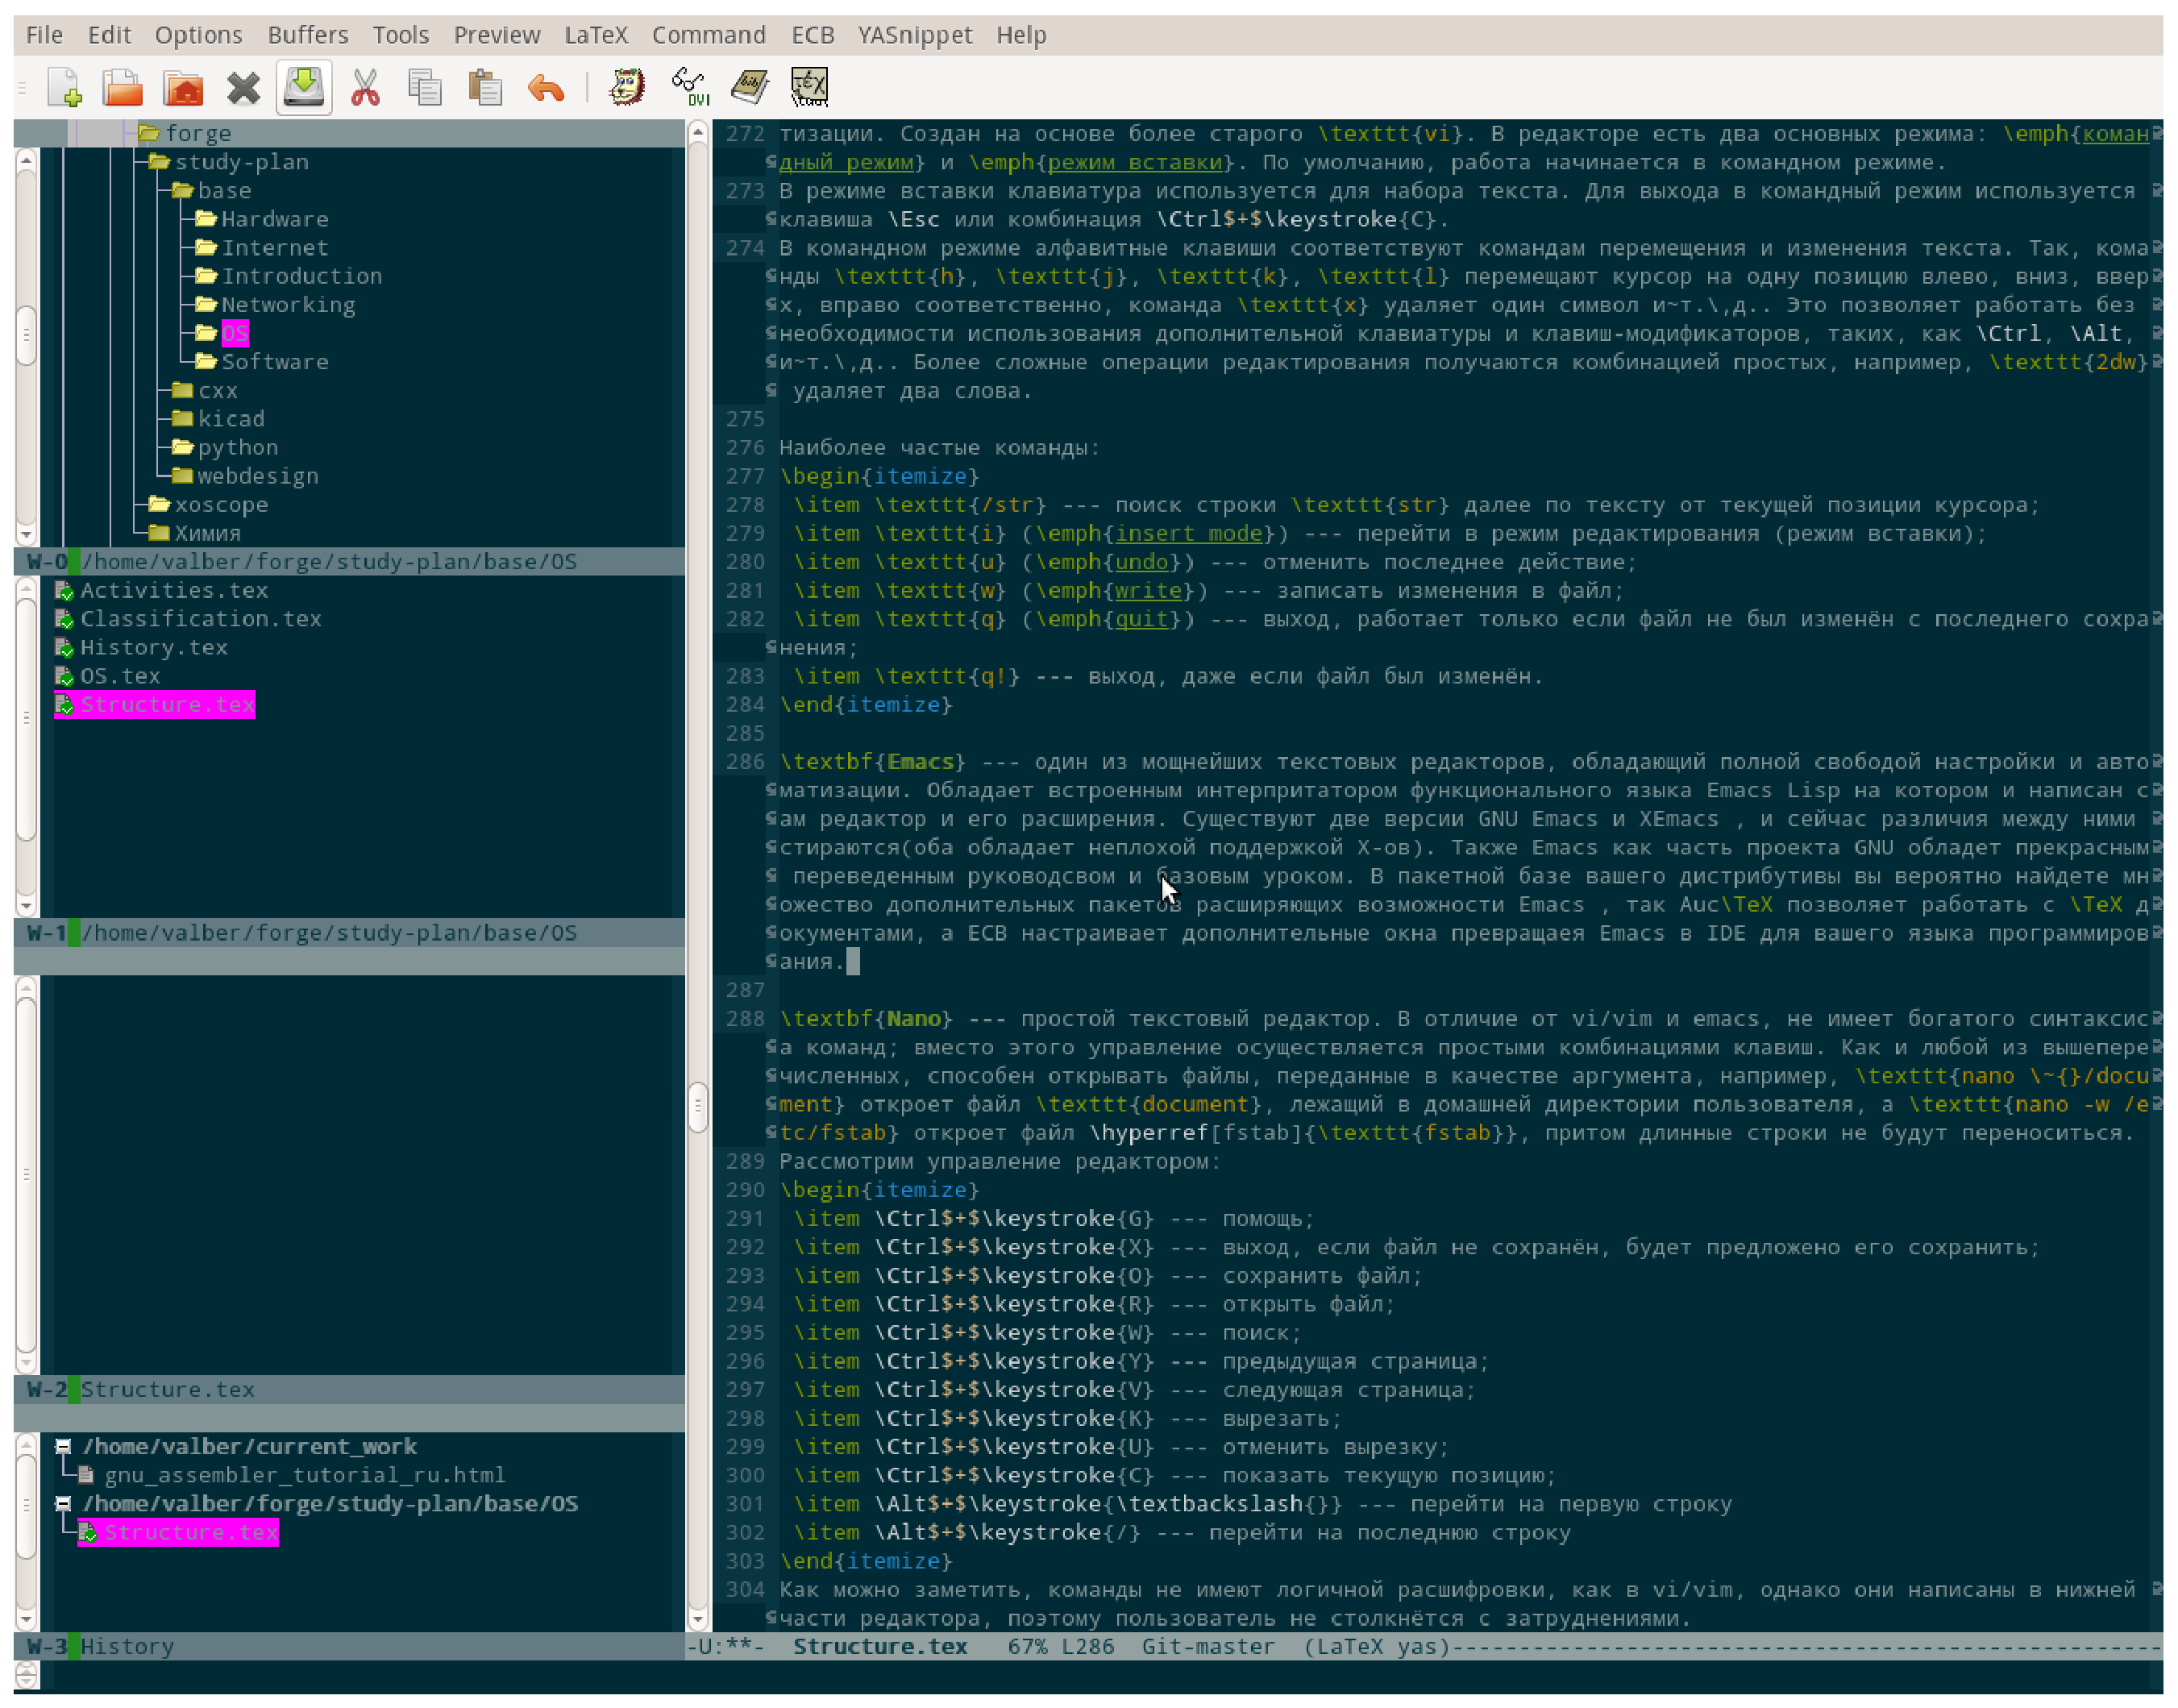
\includegraphics[scale=0.3]{base/OS/Emacs.eps}
\end{center}

Рассмотрим обозначения, если написано \Ctrl$-$\keystroke{s} это означает с зажатой клавишей \Ctrl , нажать клавишу \keystroke{s} ,а если написано  \Ctrl$-$\keystroke{x} \keystroke{1} это означает что с зажатой клавишей \Ctrl надо нажать \keystroke{x} ,затем отпустить клавишы и нажать клавишу \keystroke{1}. В руководствах и справках принято обозначение \Ctrl - \textbf{C} , \Alt - \textbf{M}. Буфер - это что-то вроде вкладок в других редакторах. Редактор не удаляет текст, а перемещает его в специальный буфер, откуда его можно будет опять вставить -это называется "убить" текст.

\begin{itemize}
  \item \Ctrl$+$\keystroke{x} \Ctrl$+$\keystroke{f}  --- открыть файл;
  \item \Ctrl$+$\keystroke{x} \Ctrl$+$\keystroke{s}  --- сохранить файл;
  \item \Ctrl$+$\keystroke{x} \Ctrl$+$\keystroke{c}  --- выход;
  \item \Ctrl$+$\keystroke{x} \keystroke{s}          --- поиск;
  \item \Ctrl$+$\keystroke{x} \keystroke{2}  --- разделить текущее окно по вертикали;
  \item \Ctrl$+$\keystroke{x} \keystroke{3}  --- разделить текущее окно по горизонтали;
  \item \Ctrl$+$\keystroke{x} \keystroke{o}  --- перейти в соседнее окно emacs;
  \item \Ctrl$+$\keystroke{x} \keystroke{b}  --- указать буфер и перети в него;
  \item \Ctrl$+$\keystroke{x} \Ctrl$+$\keystroke{b}  --- список буферов;
  \item \Ctrl$+$\keystroke{x} \keystroke{u}  --- отмена;
  \item \Ctrl$+$\keystroke{k}  --- убить строку;
  \item \Ctrl$+$\keystroke{w}  --- убить выделенный фрагмент текста;
  \item \Ctrl$+$\keystroke{y}  --- вставить последний фрагмент убитого текста;
  \item \Alt$+$\keystroke{y}   --- перелистывать после вставки назад буфер убитого текста;
  \item \Ctrl$+$\keystroke{v} или \PgDown  --- листать вниз;
  \item \Alt$+$\keystroke{v}  или \PgUp    --- листать вверх;
  \item \Ctrl$+$\keystroke{a} или \Home  --- в начало строки;
  \item \Ctrl$+$\keystroke{e} или \End   --- в конец строки;
  \item \Alt$+$\keystroke{a}  --- в начало абзаца;
  \item \Alt$+$\keystroke{e}  --- в конец абзаца;
  \item \Ctrl$+$\LArrow  --- перейти на слово влево;
  \item \Ctrl$+$\RArrow  --- перейти на слово вправо;
  \item \Ctrl$+$\BSpace  --- удалить слово слева;
  \item \Ctrl$+$\Del     --- удалить слово справа;
  \item \Ctrl$+$\keystroke{h} \keystroke{i}  --- открыть info страницы руководства;
\end{itemize}

Говорить о Emacs можно очень долго, советую пройти базовый урок, а также если вы захотите изучить какой-то редактор , необходимо запретить себе пользоваться остальными редакторами , хотя бы на время ,чтобы привыкнуть к управлению. Комбинации клавиш Emacs по перемещению и удалению текста поддерживаются многими программами, например Mozilla Firefox. Если вам понадобится среда для программирования на C  или Python с возможностью автодополнения и прочим прелестями IDE , есть неплохая уже готовая сборка \href{http://gabrielelanaro.github.com/emacs-for-python/}{emacs-for-python} , все настройки программы по умолчанию расположены в файле ~/.emacs и в каталоге ~/.emacs.d/


\textbf{Nano} --- простой текстовый редактор. В отличие от vi/vim и emacs, не имеет богатого синтаксиса команд; вместо этого управление осуществляется простыми комбинациями клавиш. Как и любой из вышеперечисленных, способен открывать файлы, переданные в качестве аргумента, например, \texttt{nano \~{}/document} откроет файл \texttt{document}, лежащий в домашней директории пользователя, а \texttt{nano -w /etc/fstab} откроет файл \hyperref[fstab]{\texttt{fstab}}, притом длинные строки не будут переноситься.
Рассмотрим управление редактором:
\begin{itemize}
 \item \Ctrl$+$\keystroke{G} --- помощь;
 \item \Ctrl$+$\keystroke{X} --- выход, если файл не сохранён, будет предложено его сохранить;
 \item \Ctrl$+$\keystroke{O} --- сохранить файл;
 \item \Ctrl$+$\keystroke{R} --- открыть файл;
 \item \Ctrl$+$\keystroke{W} --- поиск;
 \item \Ctrl$+$\keystroke{Y} --- предыдущая страница;
 \item \Ctrl$+$\keystroke{V} --- следующая страница;
 \item \Ctrl$+$\keystroke{K} --- вырезать;
 \item \Ctrl$+$\keystroke{U} --- отменить вырезку;
 \item \Ctrl$+$\keystroke{C} --- показать текущую позицию;
 \item \Alt$+$\keystroke{\textbackslash{}} --- перейти на первую строку
 \item \Alt$+$\keystroke{/} --- перейти на последнюю строку
\end{itemize}
Как можно заметить, команды не имеют логичной расшифровки, как в vi/vim, однако они написаны в нижней части редактора, поэтому пользователь не столкнётся с затруднениями.

\subsubsection{Работа с файлами}\label{base:os:structure:userutils:files}
В составе любой операционной системы общего назначения должны также находиться инструменты для работы с файлами: копирование, перемещение, удаление, переименование, работа с директориями, и~т.\,д..
Итак:
\begin{itemize}
 \item Работа с директориями:
  \begin{itemize}
   \item \texttt{pwd} (\emph{print name of current/working directory}) --- показывает текущую директорию;
   \item \texttt{cd} <\emph{dir}> (\emph{change directory}) --- сменить текущую директорию на \emph{dir};
   \item \texttt{mkdir} <\emph{dir}> (\emph{make directory}) --- создать директорию \emph{dir};
   \item \texttt{rmdir} <\emph{dir}> (\emph{remove directory}) --- удалить директорию \emph{dir}. Если директория не пуста, будет выведена ошибка;
   \item \texttt{ls} (\emph{list}) или \texttt{dir} --- вывести список файлов в текущем каталоге; если указан другой в качестве аргумента, то выводится список файлов в каталоге-аргументе. Из опций следует отметить \texttt{-h} (\emph{human readable}), выводящую информацию о размере файлов в понятной форме, и \texttt{-l} (\emph{long}), меняющую вывод с простого списка на детальную таблицу, в которой указываются права доступа, владелец, группа, размер и время создания файлов.
  \end{itemize}
 \item Получение информации о месте на разделе:
  \begin{itemize}
   \item \texttt{du} (\emph{disk usage}) --- выводит информацию об использовании диска файлами, переданными в качестве аргумента. Если аргумент опущен, выводится информация по текущему каталогу. Из полезных опций следует отметить \texttt{-h} (\emph{human readable}) --- выводить в человекочитаемой форме, и \texttt{-s} (\emph{summarize}) --- выводить информацию только по аргументу, не выводя данных обо всех вложенных файлах;
   \item \texttt{df} (\emph{disk free}) --- вывести информацию о наличии свободного места на всех дисках (если аргумент не указан) или на том, на котором располагается файл-аргумент. Следует отметить опцию \texttt{-h} (\emph{human readable}), выводящую информацию в пригодном для чтения виде.
  \end{itemize}
 \item Работа с файлами:
  \begin{itemize}
   \item \texttt{cp} <\emph{source}> <\emph{destination}> (\emph{copy}) --- скопировать файл \emph{source} в \emph{destination}. Если \emph{destination} --- обычный файл, то \emph{source} будет скопирован с именем \emph{destination}. Например:\\
    \texttt{\$ cp file1.txt file2.txt} --- скопировать \texttt{file1.txt} в эту же директорию под именем \texttt{file2.txt};\\
    \texttt{\$ cp \~{}/file1.txt ./} --- скопировать \texttt{file1.txt}, находящийся в домашнем каталоге пользователя, в текущий каталог. Имя файла останется неизменным;\\
    \texttt{\$ cp file1.txt \~{}/dir/file2.bak} --- скопировать \texttt{file1.txt}, находящийся в текущей директории, в директорию \texttt{dir/}, находящейся в домашней директории пользователя, под именем \texttt{file2.bak}.\\
   Для копирования каталогов используется ключ \texttt{-r} (\emph{recursive}):\\
    \texttt{cp -r dir \~{}/} --- скопировать директорию \texttt{dir} в домашнюю, под тем же именем;\\
    \texttt{cp -r /etc/ /mnt/backups/backup-etc} --- скопировать директорию \texttt{/etc/} в \texttt{/mnt/backups/} под именем \texttt{backup-etc}.
   \item \texttt{mv} <\emph{source}> <\emph{destination}> (\emph{move}) --- переместить \emph{source} в \emph{des\-ti\-na\-ti\-on}. Если \emph{destination} --- обычный файл, лежащий в той же директории, что и \emph{source}, будет выполнено простое переименование. Примеры использования идентичны команде \texttt{cp}, поэтому не будем на них останавливаться;
   \item \texttt{rm} <\emph{file}> (\emph{remove}) --- удаляет \emph{file}, если \emph{file} --- не директория. Ключ \texttt{-r} позволяет удалять файлы рекурсивно; таким образом можно удалять непустые директории.
  \end{itemize}
\end{itemize}

\subsubsection{Управление процессами}\label{base:os:structure:userutils:processes}
Теперь обратим внимание на такую важную вещь, как управление запущенными приложениями. Каждое приложение, как известно, при запуске создаёт свой процесс, который выполняется, пока не получит инструкцию завершения от пользователя, выполнит своё действие и завершится сам или в результате внутренней ошибки не прервёт своё выполнение.
Для управления процессами пользователю предоставлены \emph{сигналы}, которые он может послать. Каждый сигнал приводит к какому-то действию. Это:
\begin{itemize}
 \item \textbf{Term} --- завершение;
 \item \textbf{Ign} --- игнорировать сигнал;
 \item \textbf{Core} --- завершить процесс и записать дамп памяти процесса;
 \item \textbf{Stop} --- остановить процесс;
 \item \textbf{Cont} --- продолжить выполнение процесса, если он был остановлен.
\end{itemize}
Приведём список наиболее полезных с точки зрения пользователя сигналов:
\begin{itemize}
 \item \texttt{SIGTERM} --- завершить процесс, нормальное завершение;
 \item \texttt{SIGKILL} --- <<убить>> процесс, мгновенное завершение с возможной потерей данных;
 \item \texttt{SIGSTOP} --- остановить процесс;
 \item \texttt{SIGCONT} --- продолжить выполнение процесса;
 \item \texttt{SIGQUIT} --- завершить процесс и сбросить дамп памяти;
\end{itemize}
Сигналы \texttt{SIGSTOP} и \texttt{SIGKILL} не могут быть перехвачены, заблокированы или проигнорированы. В качестве примера сигнала, приводящего к \textbf{ign}, можно привести \texttt{SIGCHLD}, информирующего процесс о том, что его потомок остановил своё выполнение или завершился.

Чтобы послать сигнал используется команда \texttt{kill} с ключом \texttt{-s} \emph{SIGNAL} и PID процесса, где \emph{SIGNAL} --- сигнал, который нужно послать, например:\\
\texttt{\$ kill -s SIGSTOP 6545} --- остановить процесс с PID 6545.

Для того, чтобы посмотреть список процессов, есть программа \texttt{ps} (\emph{proccesses snapshot}). Без каких-либо опций она выведет процессы, запущенные с терминала, с которого её вызвали. При добавлении ключа \texttt{-A} она выводит список всех процессов. По-умолчанию выводятся PID процесса, терминал, с которого он был запущен, процессорное время и команду, с которой он был запущен.
Чтобы узнать PID процесса, не выводя при этом другой информации (например, если надо передать этот PID команде \texttt{kill}), можно воспользоваться опциями \texttt{-C} (выбор по команде) и \texttt{-o} (настроить вывод):\\
\texttt{\$ ps -C bash -o pid=} --- показать PID всех процессов \texttt{bash};\\
\texttt{\$ kill -s SIGSTOP `ps -C cp -o pid=`} --- остановить все процессы копирования в системе.

Каждый процесс находится в каком-то определённом состоянии, которые называются \emph{state}. Это может быть:
\begin{itemize}
 \item \textbf{D} --- непрерываемый сон, процесс в таком состоянии невозможно даже <<убить>>, послав сигнал \texttt{SIGKILL}. Как правило, процесс входит в такое состояние при ожидании ответа от дисковой подсистемы или аналогичной службы ядра;
 \item \textbf{R} --- выполняется;
 \item \textbf{S} --- прерываемый сон (ожидание окончания какого-то события)
 \item \textbf{T} --- остановлено;
 \item \textbf{W} --- подкачка страниц памяти;
 \item \textbf{X} --- мёртв (в нормальных условиях пользователь такого состояния не увидит);
 \item \textbf{Z} --- <<зомби>>-процесс, завершён, но ещё числится в потомках у своего родителя;
\end{itemize}
Если в ядре включено BSD-управление процессами, могут быть выведены также:
\begin{itemize}
 \item \textbf{<} --- процесс с высоким приоритетом;
 \item \textbf{N} --- процесс с низким приоритетом;
 \item \textbf{L} --- имеет невыгружаемые страницы памяти;
 \item \textbf{s} --- лидер сессии;
 \item \textbf{l} --- многопоточный;
 \item \textbf{$+$} --- входит в группу процессов переднего плана.
\end{itemize}
Чтобы узнать статус процесса можно добавить ключ \texttt{-u} к команде \texttt{ps}.

\subsection{Системные библиотеки}\label{base:os:structure:libs}
Чтобы не пришлось <<учить>> каждую программу как, например, открывать файл, работать с потоками или совершать иные частоиспользуемые действия, многие операции выносятся в \emph{библиотеки}. Они содержат определённый набор готовых функций, которыми может воспользоваться любая программа, таким образом время разработки уменьшается и стабильность приложений растёт. Библиотеки, которыми пользуются системные утилиты, называются \emph{системными}.

Библиотеки располагаются в каталогах \texttt{/lib/}, \texttt{/usr/lib/}, и \texttt{/usr/lo\-cal/lib/}. Для <<базовой>> системы достаточно \texttt{/lib/}. Там же находятся модули ядра.
% Надо ли ещё что-то указывать?

\subsection{Командная оболочка}\label{base:os:structure:shell}
Для взаимодействия с пользователем, как уже известно, используются определённые команды (\hyperref[base:introduction:control]{глава \ref*{base:introduction}, раздел \ref*{base:introduction:control}}).
Для интерпретации этих команд служат \emph{командные интерпретаторы}, или \emph{командные оболочки}. В операционные системы MS-DOS и Windows 9x включён командный интерпретатор \texttt{command.com}, в Windows NT включён \texttt{cmd.exe}, начиная с Windows XP (пакет обновления 2) доступен \emph{PowerShell}, который является встроенным компонентом ОС начиная с Windows 7 и Windows 2008 Server.

В большом семействе командных оболочек UNIX наиболее популярны \emph{bash}, \emph{csh}, \emph{ksh}, \emph{zsh}. Также в UNIX-подобных системах у пользователя есть возможность менять командный интерпретатор, используемый по умолчанию.

\subsubsection{Функции}
Командный интерпретатор исполняет команды своего языка, заданные в командной строке или поступающие из стандартного ввода или указанного файла.

В качестве команд интерпретируются вызовы системных или прикладных утилит, а также управляющие конструкции. Кроме того, оболочка отвечает за раскрытие шаблонов имен файлов и за перенаправление и связывание ввода-вывода утилит.

В совокупности с набором утилит, оболочка представляет собой операционную среду, язык программирования и средство решения как системных, так и некоторых прикладных задач, в особенности, автоматизации часто выполняемых последовательностей команд.
% Потом дополню ещё чем-нить

\subsection{Система документации}\label{base:os:structure:docs}
\subsubsection{Средства операционной системы}
В большинстве случаев вместе с системой поставляется также механизм получения справки по встроенным командам, приложениям и прочему. В POSIX-совместимых системах за это отвечают приложения \texttt{/usr/bin/man} и \texttt{/usr/bin/info}. \texttt{man} по историческим причинам более популярна, поэтому остановимся на ней.

При вызове справки через программу \texttt{man} (например, \texttt{man man}) происходит поиск \emph{man-страниц} в директориях, указанных в переменной \texttt{MANPATH}. По умолчанию эта переменная заполняется значениями, указанными в конфигурационном файле \texttt{/etc/man.conf}, однако может быть дополнена или изменена пользователем.

При использовании пользователь может указать раздел, из которого требуется информация. Это может быть:
\begin{enumerate}
 \item описание команд пользователя;
 \item описание системных вызовов;
 \item функции стандартной библиотеки Си;
 \item информация об устройствах и специальных файлах;
 \item игры;
 \item разная информация, не попадающая под другие разделы;
 \item инструменты администрирования системы, такие как утилиты и демоны.
\end{enumerate}
Если номер раздела не указывается, используется младший доступный.
Например, вызов \texttt{man signal} эквивалентен \texttt{man 2 signal}. Оба выведут информацию о работе с сигналами в языке Си. Однако \texttt{man 7 signal} покажет обзор сигналов как таковых с описанием их действий и списком возможных сигналов.

\subsubsection{Внутренняя справка приложений}
Также информация о том, как пользоваться программами зачастую встроена в них самих. В POSIX-совместимых системах для вызова справки (правда, зачастую куда менее подробной, нежели man- и info-стра\-ни\-цы) нужно добавить ключ \texttt{-\text{-}help}, например \texttt{cp -\text{-}help} вызовет основы использования программы \hyperref[base:os:structure:userutils:files]{\texttt{cp}}. В DOS-совместимых системах для этих же целей используется ключ \texttt{/?}.

\subsection{Дополнительные компоненты}\label{base:os:structure:additional}
Этот список можно дополнить двумя опциональными, но практически столь же обязательными пунктами:

\subsubsection{Набор средств установки пакетов}\label{base:os:structure:additional:packagemanager}
В стандартной поставке дистрибутивы операционных систем обеспечивают некоторую функциональность, но зачастую её недостаточно (а у некоторых дистрибутивов, особенно рассчитанных на опытных пользователей, такого понятия как <<стандартная установка>> попросту нет). Поэтому возникает необходимость расширить эту функциональность посредством установки различного ПО.
Притом нужно учитывать, что различным программам могут требоваться определённые библиотеки, которых нет в системе, а иногда и другие приложения, у которых могут быть свои зависимости. Также не следует забывать о размещении файлов, чтобы не получить ситуацию, когда одна программа при установке перезаписала файлы другой.
В дистрибутивах GNU/Linux, семействе BSD и некоторых других системах за этим следит т.\,н. пакетный менеджер (APT, RPM, pacman, emerge), через который и происходит установка, удаление и обновление ПО. В системах microsoft (Windows\texttrademark, DOS) установка приложений и разрешение возможных конфликтов ложится на пользователя, поэтому обычно каждое приложение располагается в своей поддиректории. Подробнее управление пакетами в различных системах будет рассмотрено \hyperref[base:software:packages]{в главе \ref*{base:software}, раздел \ref*{base:software:packages}}.

\subsubsection{Система поддержки работы в графическом режиме}\label{base:os:structure:additional:gui}
Хотя для большинства задач это необязательно (например, смотреть фильмы, слушать музыку, посещать web-страницы и прочее можно делать в консоли), всё-таки есть области, для которых поддержка графического режима необходима, например, 3D-моделирование. Также для многих операций управление через GUI просто приятнее и удобнее.

Системы графического интерфейса будут рассмотрены \hyperref[base:software:de]{в главе \ref*{base:software} раздел \ref*{base:software:de}} и в последующих.